\documentclass[12pt,oneside]{settingsTemplate}
\AtBeginDocument{\RenewCommandCopy\qty\SI}
%load any additional packages

%\usepackage{mathptmx}  % Usa Times (simile a Times New Roman)
%\renewcommand{\rmdefault}{ptm}  % Imposta il font principale su Times
%\renewcommand{\bfdefault}{b}  % Usa la variante grassetto di Times

\usepackage{algorithm}
\usepackage{algorithmicx}
\usepackage{algpseudocode}
\usepackage{amsmath}
\usepackage{amssymb}
\usepackage[italian]{babel}
\usepackage{booktabs}
\usepackage{dirtree}
\usepackage[T1]{fontenc}
\usepackage[a4paper]{geometry}
\usepackage[utf8]{inputenc}
\usepackage{mathtools}
\usepackage{multirow}
\usepackage{physics}
\usepackage[binary-units]{siunitx}
\usepackage{textcomp}
\usepackage{xcolor}
\usepackage{hyperref}
\usepackage{tabularx}
\usepackage{titlesec}
\usepackage{enumitem}
\usepackage{amsmath} % Per la modalità matematica avanzata
\usepackage{amsfonts} % Per \mathbb


\hypersetup{
    colorlinks=false,
    pdfborder={0 0 0}
}

\usepackage[toc,acronym,nomain,nonumberlist,nopostdot]{glossaries}
\usepackage{caption}
\usepackage{subcaption}
\expandafter\def\csname ver@subfig.sty\endcsname{}
\AtBeginDocument{\RenewCommandCopy\qty\SI}
% \ExplSyntaxOn
% \msg_redirect_name:nnn{siunitx}{physics-pkg}{none}
% \ExplSyntaxOff
\usepackage[binary-units=true]{siunitx}

\usepackage{soul}
\usepackage{pdfpages}
\usepackage{tabularx}
\usepackage{subfig}
\usepackage{graphicx}

\usepackage{array}

%\usepackage{mdframed}
\usepackage{xcolor}

% to debug sheet sizes
%\usepackage{layout}
%\usepackage{showframe}
% then use \layout{} in your document environment to show measures

% algorithm package configuration
\makeatletter
\def\BState{\State\hskip-\ALG@thistlm}
\makeatother

%note \\[1ex] can be a line break in the title
\title{Titolo Dell'Elaborato}

\author{Nome \scshape Cognome}

%professor names can be changed from the file "settingsTemplate.cls"

\department{Dipartimento di Ingegneria Elettrica e dell'Informazione}
\university{Politecnico Di Bari}


\renewcommand{\submittedtext}{Tesi di Laurea in}
\renewcommand{\course}{XX}
\degree{Triennale/Magistrale in  \\ XX}

\makeglossaries
\setacronymstyle{long-short}


%end the preamble and start the document
\begin{document}
\newacronym{dei}{DEI}{Dipartimento di Ingegneria Elettrica e dell’Informazione}
\newacronym{sigla1}{SIGLA1}{Inserire qui la denominazione della sigla o abbreviazione}
\newacronym{sigla2}{SIGLA2}{Testo dell'altra sigla}
%this baselineskip gives sufficient line spacing for an examiner to easily
%markup the thesis with comments
\baselineskip=18pt plus1pt

%set the number of sectioning levels that get number and appear in the contents
\setcounter{secnumdepth}{3} %Mostra numerazione fino a \subsubsection
\setcounter{tocdepth}{2}  % Include fino al \subsection nell'indice

\maketitle                  % create a title page from the preamble info
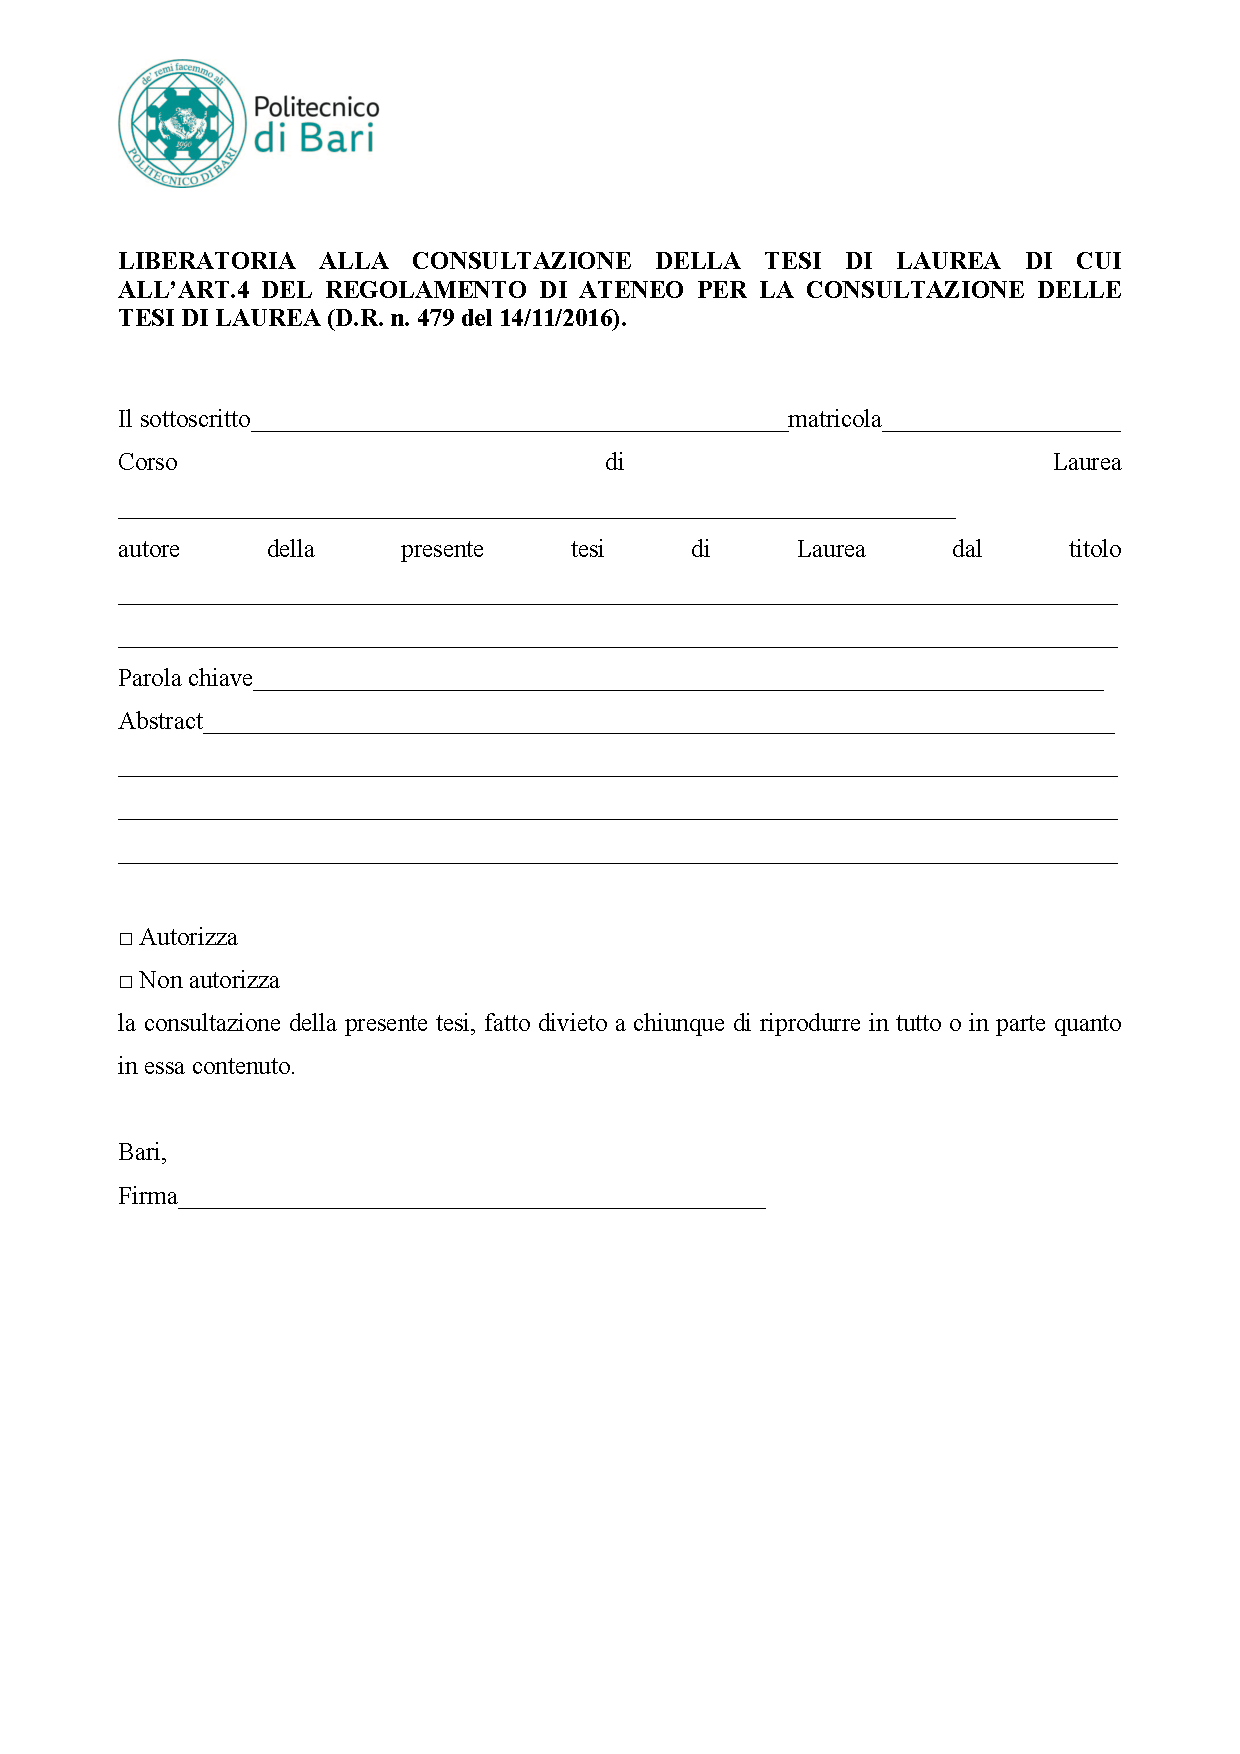
\includepdf[pages=-]{LIBERATORIA_TESI.pdf}
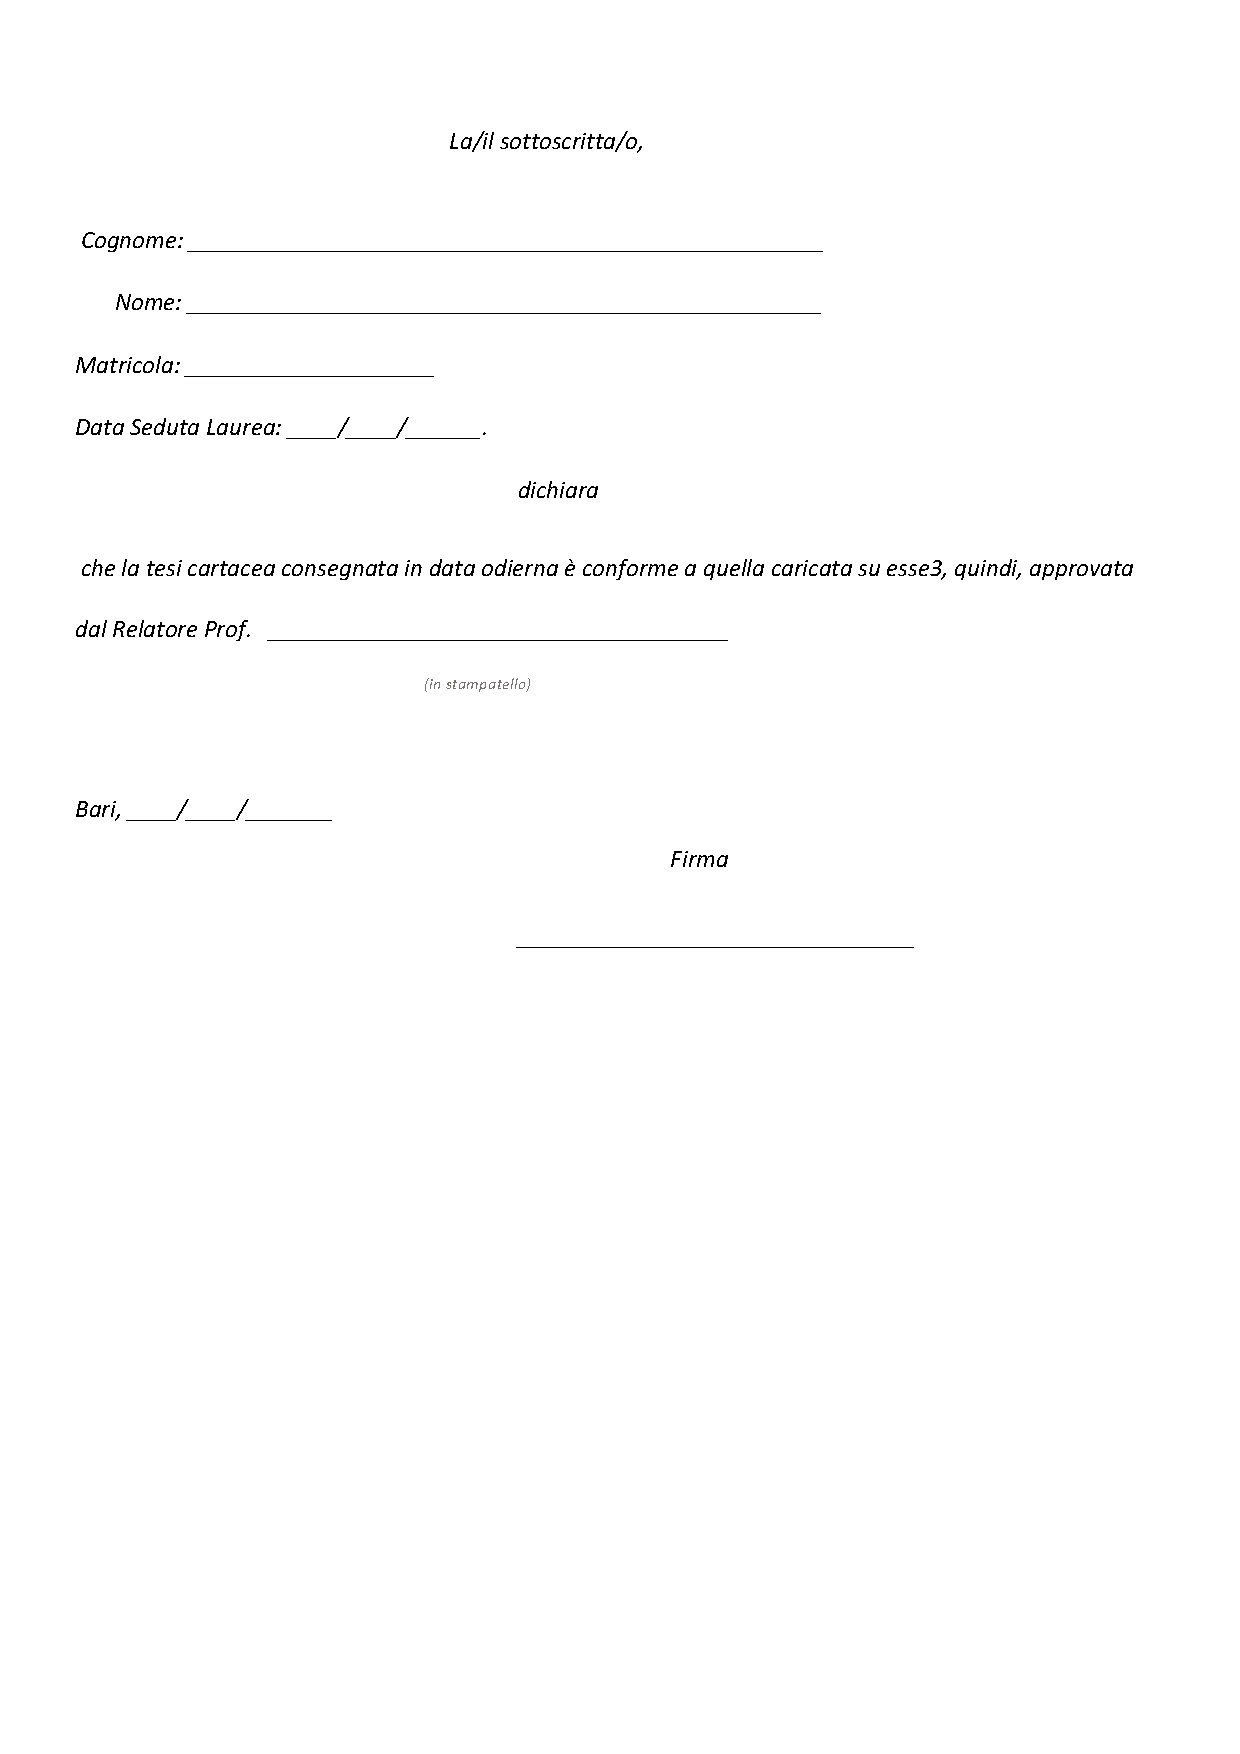
\includepdf[pages=-]{Dichiarazione-Tesi-Conforme.pdf}

\pagenumbering{gobble} % Nasconde la numerazione iniziale



\begin{flushright}
    \textit{
        Inserire qui l’eventuale dedica. \\
        Questo è un esempio di capoverso che serve per mostrare \\
        le caratteristiche dello stile “Dedica”.\\
        Usare l’interruzione di riga forzata (SHIFT+INVIO) \\
        per mantenere unite le righe.
    }
\end{flushright}        % include a dedication.tex file
% \include{acknowlegements}   % include an acknowledgements.tex file
\include{abstract}          % include the abstract
%\begin{romanpages}          % start roman page numbering
\renewcommand{\contentsname}{\scshape Indice} %mette il titolo in maiuscoletto
\tableofcontents
%\end{romanpages}            % end roman page numbering

\renewcommand{\listtablename}{\scshape Elenco delle Tabelle} % modify the title of the list of tables
\addcontentsline{toc}{chapter}{\scshape \listtablename} %mostra il titolo in maiuscoletto nell'indice
\listoftables

\pagenumbering{arabic} % Fa ripartire la numerazione delle pagine
\setcounter{page}{1} % Imposta il numero di pagina a 1


%Inizio Script per spostare il numero in basso a destra
\makeatletter
\renewcommand{\ps@plain}{%
    \renewcommand{\@oddfoot}{\mbox{}\hfill\thepage} % Numero in basso a destra
    \renewcommand{\@evenfoot}{\mbox{}\hfill\thepage} % Per pagine pari
}
\makeatother
\pagestyle{plain} % Applica il nuovo stile modificato
%Fine Script per spostare il numero in basso a destra


\renewcommand{\listfigurename}{\scshape Elenco delle Figure} % modify the title of the list of figures
\addcontentsline{toc}{chapter}{\scshape \listfigurename} %mostra il titolo in maiuscoletto nell'indice
\listoffigures

%\printglossaries
\printglossary[type=acronym, title={\scshape Acronimi e Abbreviazioni}] %modify the name of the glossary

%now include the files of latex for each of the chapters etc
\chapter*{\scshape Introduzione e Scopo della Tesi}
\addcontentsline{toc}{chapter}{\scshape Introduzione e Scopo della Tesi} %this line allows that the introduction could be in the table of contents

Inserire qui il testo dell’introduzione.
\chapter{\scshape Titolo del Capitolo: è un esempio per mostrare lo stile "Capitolo"}

Inserire qui il testo del capitolo. Questo è un esempio di capoverso che serve per mostrare le caratteristiche dello stile del corpo del testo (“Normale”). \\

Questo è il Template delle Tesi di Laurea del \gls{dei}. Come potete vedere, il testo al passaggio del mouse si evidenzia di giallo e questo mostra l'inserimento di un acronimo, visibile al click nella pagina "Acronimi e Abbreviazioni". La creazione di un nuovo acronimo la puoi vedere all'interno del file "acronyms.tex". \\

Di seguito altri esempi di Acronimi e Abbreviazioni: \\
\begin{itemize}
    \item \gls{sigla1}
    \item \gls{sigla2}
\end{itemize}

\section{Sotto capitolo: questo è un esempio di titolo che serve per mostrare le caratteristiche dello stile “Titolo 2”}

Inserire qui il testo del sotto capitolo. Questo è un esempio di citazione bibliografica in stile IEEE \cite{id1}. 

\textbf{Per creare una citazione (su Microsoft Word)}:  
\begin{enumerate}
    \item posizionare il cursore nel punto del testo in cui si desidera inserire la citazione;
    \item nella barra Riferimenti > Citazioni e bibliografia > Stile scegliere lo stile IEEE;
    \item passare a Riferimenti > Inserisci citazione e scegliere l’origine citazione. In alternativa scegliere Aggiungi nuova fonte e compilare le informazioni dell'origine.
\end{enumerate} 

\textbf{Per creare una citazione (su Overleaf con LaTeX)}:
\begin{enumerate}
    \item vai nel file "bibliography.tex";
    \item creare una citazione con la @ (come ad esempio @article);
    \item riempire tutti i campi;
    \item posizionare il cursore nel punto del testo in cui si desidera inserire la citazione;
    \item scrivere "\verb|\|cite\{\}" con all'interno delle parentesi graffe l'id della citazione (nell'esempio riportato precedentemente è "id1").
\end{enumerate}



\begin{quote}
    «Inserire qui il testo della citazione lunga (almeno 4-5 righe). Questo è un esempio di capoverso che serve per mostrare le caratteristiche dello stile delle citazioni lunghe (“Citazione”).»
\end{quote}



\noindent \textbf{Per inserire una nota a piè di pagina (su Microsoft Word)}:
\begin{enumerate}
    \item selezionare la parola di cui si vuole creare la nota; 
    \item nella barra Riferimenti > Note a piè di pagina > Inserisci nota a piè di pagina.
\end{enumerate}

\noindent \textbf{Per inserire una nota a piè di pagina (su Overleaf con LaTeX)}:
\begin{enumerate}
    \item posizionarsi con il cursore del mouse dove si vuole inseire la nota a piè di pagina;
    \item scrivere "\verb|\|footnote\{\}" con all'interno delle parentesi graffe l'id della citazione (nell'esempio riportato successivamente è "Questa è la nota a piè di pagina.").
\end{enumerate}

Questo è un esempio di testo con una nota a piè di pagina\footnote{Questa è la nota a piè di pagina.}

\subsection{Titolo del sotto-sotto capitolo: questo è un esempio di titolo che serve per mostrare le caratteristiche dello stile “Titolo 3”}

Inserire qui il testo del sotto-sotto capitolo.

Questo è un esempio di citazione che ha come fonte una pagina WEB in stile IEEE \cite{id2}. 

\textbf{Per creare una citazione che ha come fonte una pagina WEB (su Microsoft Word)}:
\begin{enumerate}
    \item posizionare il cursore nel punto del testo in cui si desidera inserire la citazione;
    \item nella barra Riferimenti > Citazioni e bibliografia > Stile scegliere lo stile IEEE;
    \item passare a Riferimenti > Inserisci citazione e scegliere l’origine citazione. In alternativa scegliere Aggiungi nuova fonte e selezionare in Tipo di fonte: “Sito Web” e inserire le informazioni del sito web includendo URL.
\end{enumerate} 

\textbf{Per creare una citazione che ha come fonte una pagina WEB (su Overleaf con LaTeX)}:
\begin{enumerate}
    \item vai nel file "bibliography.tex";
    \item creare una citazione con la @ (come ad esempio @misc);
    \item riempire tutti i campi;
    \item posizionare il cursore nel punto del testo in cui si desidera inserire la citazione;
    \item scrivere "\verb|\|cite\{\}" con all'interno delle parentesi graffe l'id della citazione (nell'esempio riportato precedentemente è "id2").
\end{enumerate}

\subsubsection{Sotto-sotto-sotto capitolo: questo è un esempio di titolo che serve per mostrare le caratteristiche dello stile “Titolo 4”}

Inserire qui il testo del sotto-sotto-sotto capitolo.
\chapter{\scshape Titolo del Capitolo}

Inserire qui il testo del capitolo

\section{Titolo del sotto capitolo}
Inserire qui il testo del sotto capitolo. \\

\noindent Di seguito è riportato un esempio di Tabella. 

Per inserire la tabella con la sua didascalia su Overleaf con LaTeX guardare il codice del documento.

Per inserire la didascalia alla tabella su Microsoft Word: 
\begin{enumerate}
    \item fare clic sulla tabella;
    \item fare clic su Riferimenti > Inserisci didascalia; 
    \item selezionare l’etichetta Tabella, la posizione Sopra l’elemento selezionato.
\end{enumerate} 

La didascalia utilizza lo stile “Didascalia”. Formattare le tabelle come indicato (Times New Roman 11 pt; Spaziatura prima e dopo 1 pt).  \\

Evitare linee verticali a meno che non siano strettamente necessarie e funzionali ad una migliore comprensione dei dati riassunti nella tabella.

È importante che tutte le tabelle inserite siano citate almeno una volta nel corpo del testo.

\begin{table}[H]
    \centering
    %\begin{tabular}{c c c c}
    \begin{tabular*}{\textwidth}{@{\extracolsep{\fill}} c c c c c @{}}
        \hline
        \textbf{} & \textbf{Colonna 2} & \textbf{Colonna 3} & \textbf{Colonna 4} & \textbf{Colonna 5}\\
        \hline
        Riga 1 &  &  &  &\\
        %\hline
        Riga 2 &  &  &  &\\
        %\hline
        Riga 3 &  &  &  &\\
        %\hline
    %\end{tabular}
    \end{tabular*}
    \caption{Titolo della Tabella}
    \label{tab:esempio-tabella}
\end{table}

\begin{table}[H]
    \centering
    \begin{tabular}{c c c c c}
        \hline
        \textbf{} & \textbf{Colonna 2} & \textbf{Colonna 3} & \textbf{Colonna 4} & \textbf{Colonna 5}\\
        \hline
        Riga 1 &  &  &  &\\
        %\hline
        Riga 2 &  &  &  &\\
        %\hline
        Riga 3 &  &  &  &\\
        %\hline
    \end{tabular}
    \caption{Titolo della Tabella 2}
    \label{tab:esempio-tabella-2}
\end{table}

\subsection{Titolo del sotto-sotto capitolo}
Inserire qui il testo del sotto-capitolo


\chapter{\scshape Titolo del Capitolo}

Inserire qui il testo del capitolo

\section{Titolo del sotto capitolo}
Inserire qui il testo del sotto capitolo.

Quello di seguito è un esempio di Figura.  \\

\noindent \textbf{Per inseire un'immagine su Overlaef con LaTeX} e con la sua didascalia basta caricare le immagini nella cartella "images" e poi seguire il codice riportato. \\

\noindent \textbf{Per inserire un’immagine su Microsoft Word} scegliere Inserisci > Immagini. \\

Utilizzare immagini di risoluzioni e dimensioni adeguate. \\

\noindent \textbf{Per inserire la didascalia su Microsoft Word}: 
\begin{enumerate}
    \item fare clic sulla figura; 
    \item fare clic su Riferimenti > Inserisci didascalia; 
    \item selezionare l’etichetta Figura, la posizione Sotto l’elemento selezionato.
\end{enumerate} 

La didascalia utilizza lo stile “Didascalia”. È importante che tutte le figure inserite siano citate almeno una volta nel corpo del testo. \\

\noindent \textbf{Per citare il riferimento della figura (Figura 1) su Microsoft Word nel corpo del testo}: 
\begin{enumerate}
    \item posizionare il cursore nel punto del testo in cui si desidera inserire la citazione alla figura; 
    \item fare clic su Inserisci > Collegamenti > Riferimento incrociato;
    \item selezionare il tipo: Figura, Inserisci riferimento a: Solo etichetta e numero;
    \item fare clic su Inserisci. 
\end{enumerate} 

\noindent \textbf{Per citare il riferimento della figura (Figura \ref{tab:esempio-immagine}) su Overleaf con LaTeX nel corpo del testo}:
\begin{enumerate}
    \item iserire l'immagine come spiegato precedentemente;
    \item aggiungere il campo "\verb|\|label\{\}";
    \item posizionare il cursore nel punto del testo in cui si desidera inserire la citazione alla figura;
    \item scrivere "\verb|\|ref\{\}" e all'interno delle parentesi graffe cioò che è stato inserito al'interno del campo "\verb|\|label\{\}" citato in precedenza.
\end{enumerate}


\begin{figure}[H]
    \centering
    
\includegraphics[width=0.7\linewidth]{images/logo-politecnico-di-bari-esteso.png}
    \caption{Esempio di Didascalia di Figura}
    \label{tab:esempio-immagine}
\end{figure}


\subsection{Titolo del sotto-sotto capitolo}
Inserire qui il testo del sotto-capitolo.\\

\noindent \textbf{Per inserire un'equazione su Overleaf con LaTeX}:
\begin{enumerate}
    \item posizionare il cursore nel punto del testo in cui si desidera inserire la citazione alla figura;
    \item inserire il tag \verb|\|begin\{equation\};
    \item iniziare a scrivere la formula seguendo le regole base di LaTeX.
\end{enumerate}

\noindent \textbf{Per inserire un'equazione su Microsoft Word}: 
\begin{enumerate}
    \item selezionare la tabella sottostante contenente l’equazione;
    \item copiare e Incollare dove necessario;
    \item cambiare il numero di riferimento dell’equazione;
    \item inserire il riferimento dell’equazione nel corpo del testo manualmente in parentesi tonde.
\end{enumerate}

È importante che tutte le equazioni inserite siano citate almeno una volta nel corpo del testo. \\

\textbf{N.B.} La tabella dell'equazione su Microsoft Word sottostante non presenta i bordi (selezionare Struttura tabella > Bordi > Nessun Bordo) ed è formata da due colonne: la prima colonna contiene l’equazione allineata al centro e inserita tramite il procedimento Inserisci > Equazione; la seconda colonna contiene il numero del riferimento in parentesi tonde ed è larga circa 1cm.

\begin{equation}
    \left(\frac{R_e}{1-D}-\frac{DT_s}{C_e}\right) \le \Delta v_{pp}^{max}
\end{equation}
\chapter*{\scshape Conclusioni}
\addcontentsline{toc}{chapter}{\scshape Conclusioni} %this line allows that the introduction could be in the table of contents


Inserire qui il testo delle conclusioni.


%next line adds the Bibliography to the contents page
\renewcommand{\bibname}{\scshape Bibliografia e Sitografia} %modify the title of the bibliography
\addcontentsline{toc}{chapter}{\scshape \bibname}
\bibliographystyle{unsrt}
\bibliography{bibliography}


%next line adds Acknowledgments to the contents page
\chapter*{\scshape Ringraziamenti}
\addcontentsline{toc}{chapter}{\scshape Ringraziamenti}

\chapter*{\scshape Istruzioni per l'Uso del Modello di Tesi}

Al termine dell’elaborazione della tesi, cancellare le seguenti istruzioni. \\ \\


\textbf{\scshape Parametri di riferimento del presente documento} \\

\textbf{Margini del documento}: sinistro 3 cm; destro 3 cm; rilegatura 0,5 cm; superiore 3 cm; inferiore 3,5 cm \\

\textbf{Numeri di pagina}: in basso a destra (frontespizio, deliberatoria, dedica, indice non sono numerate) \\ \\ \\

\textbf{\scshape Principali stili adottati} \\
la raccolta di stili completa è visibile cliccando su \textbf{Stili}\\

\textbf{\textit{Stili di paragrafo (il testo)}}\\

\textbf{Normale}: da usare per il corpo del testo; carattere Times New Roman; corpo 11 pt; interlinea 1,5; rientro prima riga 0,5 cm; nessuna spaziatura prima e dopo; giustificato. \\

\textbf{Citazione}: da usare per le citazioni lunghe (almeno 4-5 righe); carattere come il corpo del testo; corpo 11 pt; interlinea singola; rientro prima riga assente; rientro a sinistra e a destra 0,5 cm; spaziatura prima 6 pt, dopo 12 pt; giustificato. \\

\textbf{Abbreviazioni}: da usare per le sigle e le abbreviazioni nella tavola iniziale; carattere come il corpo del testo; corpo 11 pt; interlinea 1,5; prima riga sporgente di 2 cm; spaziatura dopo 6 pt; giustificato; mantieni assieme le righe. \\

\textbf{Didascalia}: da usare per le figure/tabelle; carattere come il corpo del testo; corpo 10 pt; giustificato.
Bibliografia: da usare per bibliografia/sitografia; carattere come il corpo del testo; corpo 11 pt; giustificato; Sporgente 0,5 cm, Spazio Dopo: 6 pt.\\

\textit{\textbf{Stili di paragrafo (i titoli)}} \\

\textbf{Capitolo}: da usare per i titoli delle parti principali del testo (indice, elenco delle tabelle/figure, acronimi e abbreviazioni, introduzione e scopo della tesi, capitoli, conclusioni, bibliografia, sitografia, ringraziamenti); carattere come il corpo del testo; corpo 16 pt; interlinea singola; rientro prima riga assente; spaziatura dopo 96 pt; allineamento centrato; anteponi interruzione (affinché il titolo cominci con l’inizio di una pagina); maiuscoletto. \\

\textbf{Titolo 2}: da usare per i titoli dei paragrafi; carattere come il corpo del testo; corpo 12 pt; grassetto; interlinea singola; prima riga sporgente di 0,5 cm; spaziatura prima 24 pt, dopo 12 pt; allineamento a sinistra; mantieni con il successivo; mantieni assieme le righe. \\

\textbf{Titolo 3}: da usare per i titoli dei sottoparagrafi; carattere come il corpo del testo; corpo 11 pt; corsivo; interlinea singola; prima riga sporgente di 0,5 cm; spaziatura prima 12 pt, dopo 12 pt; allineamento a sinistra; mantieni con il successivo; mantieni assieme le righe. \\

\textbf{NB}: I titoli dei capitoli, dei paragrafi e dei sottoparagrafi sono numerati automaticamente in modo strutturato (1, 1.1, 1.1.1, 1.1.1.1). La numerazione dei capitoli prevede la dicitura automatica “Capitolo 1”, “Capitolo 2”, ecc. Nell’indice, elenco delle tabelle/figure, acronimi e abbreviazioni, introduzione e scopo della tesi, conclusioni, bibliografia, sitografia, ringraziamenti, indice, la numerazione è stata eliminata. \\ \\ \\

\textbf{\scshape Bibliografia e sitografia} \\
La lista dei riferimenti bibliografici alla fine del documento è generata con il comando \textbf{Riferimenti > Bibliografia > Inserisci bibliografia}. È possibile aggiornare la lista posizionando il cursore nel punto del testo della bibliografia, premendo pulsante destro mouse, \textbf{Aggiorna campo}.\\  \\ \\

\textbf{\scshape Lista delle tabelle}\\
La lista delle tabelle è generata con il comando \textbf{Riferimenti > Inserisci indice delle figure}. Nella finestra di dialogo selezionare \textbf{Etichetta didascalia: Tabella}. È possibile aggiornare la lista posizionando il cursore nel punto del testo della lista delle tabelle, premendo pulsante destro mouse, \textbf{Aggiorna campo}.  \\ \\ \\

\textbf{\scshape Lista delle figure} \\
La lista delle figure è generata con il comando \textbf{Riferimenti > Inserisci indice delle figure}. Nella finestra di dialogo selezionare \textbf{Etichetta didascalia: Figura}. È possibile aggiornare la lista posizionando il cursore nel punto del testo della lista delle figure, premendo pulsante destro mouse, \textbf{Aggiorna campo}.  \\ \\ \\

\textbf{\scshape Indice} \\
L’indice è generato con il comando \textbf{Riferimenti > Sommario > Sommario personalizzato}. Nella finestra di dialogo selezionare \textbf{Formati: Da modello}. È possibile aggiornare la lista posizionando il cursore nel punto del testo dell’indice, premendo pulsante destro mouse, \textbf{Aggiorna campo}.
 %comment this section when you write your thesis

\end{document}